\documentclass[times, utf8, diplomski]{fer}
\usepackage{booktabs}
\usepackage{pdfpages}
\usepackage{subfiles}
\usepackage{float}

\begin{document}

% TODO: Navedite broj rada.
\thesisnumber{959}

% TODO: Navedite naslov rada.
\title{Aplikacija za interaktivnu pomoć penjačima po stijenama uporabom proširene stvarnosti}

% TODO: Navedite vaše ime i prezime.
\author{Adrian Cvijanović}

\maketitle

% Ispis stranice s napomenom o umetanju izvornika rada. Uklonite naredbu \izvornik ako želite izbaciti tu stranicu.
% \includepdf[pages=-]{izvornik.pdf}

% Dodavanje zahvale ili prazne stranice. Ako ne želite dodati zahvalu, naredbu ostavite radi prazne stranice.
\zahvala{}

\tableofcontents

\chapter{Uvod}

Digitalna tehnologija obuhaća gotovo sve aspekte ljudskog života, od komunikacije, poslovanja do zabave i znanja. Rekreativne aktivnosti i sportovi koji su se oslanjali na fizičku opremu i materijale sve više usvajaju digitalne alate koji proširuju mogućnosti i količinu informacija koje korisnici mogu dobiti. Sportsko penjanje, kao aktivnost koja spaja fizičku spremnost i boravak u prirodi, predstavlja primjer aktivnosti koja se može proširiti digitalnim alatima.

Dok su postojeće digitalne platforme omogućile lak pristup informacijama penjačkih lokacija, ključni izazov ostaje upotreba tih informacija u stvarnom okruženju - isprijed same stijene. Taj ključni izazov otvara prostor za inovacije, posebice u domeni mobilnih tehnologija, računalnog vida i proširene stvarnosti.

\section{Kontekst i rast popularnosti sportskog penjanja} 

Sportsko penjanje i srodna disciplina \textit{bouldering} posljednjih su desetljeća doživjeli eksponencijalni rast u popularnosti, Privlačeći sve veći broj entuzijasta kako u specijalizirane dvorane, tako i na prirodne stijene. Na Olimpijskim igrama 2020. godine u Tokiju sportsko penjanje je po prvi put uvršten u program čime je sport dobio globalnu pozornost i dodatno potaknuo interes javnosti. Olimpijskim igrama 2024. godine u Parizu popularnost sporta je još više porasla. Prema članku iz \textit{The Oxford Blue}, dok se vrijednost globalnod tržišta penjačkih dvorana procjenjuje na 117.61 milijardi dolara do 2031. godine \cite{the_oxford_blue_rock_climb}. S rastom zajednice, raste i potreba za kvalitetnim, dostupnim i preciznim informacijama o penjalištima i smjerovima.

\section{Problem identifikacije penjačkih smjerova i ograničenja tradictionalnih alata}

Tradicionalno, glavni izvor informacija za penjače su tiskani penjački vodiči. Ovi vodiči sadrže detaljne opise penjališta, karte pristupa, kao i skicirane prikaze stijene ili često nazivane \textit{topo} s ocrtanim linijama penjačkih smjerova, njihovim nazivima i težinama. Iako su desetljećima bili nezamjenjiv alat, tiskani vodiči imaju ograničenja. Podložni su zastarijevanju jer ne mogu pratiti dinamiku promjena na penjalištima poput dodavanja novih smjerova, promjena težina ili upozorenja o opasnostima na pojedinim smjerovima. Bilo kakve promjene zahtjevaju novo tiskanje i kupovanje novog izdanja. Tiskani vodiči su nepraktični za nošenje, a najveći izazov predstavlja interpretacija dvodimenzionalnih skica, koje su često slikane iz daljine, na trodimenzionalnu strukturu stijene. Proces lociranja točnog početka smjera na temelju crteža često je subjektivan, dugotrajan i može dovesti do frustracija ili pokušaj penjanja smjera koji je težinski izvan dohvata za penjača. 

\begin{figure}[H]
    \centering
    \includegraphics[width=0.8\textwidth]{images/uvod/tradicionalni_vodic.jpg}
    \caption{Prikaz tiskanog penjačkog vodiča}
\end{figure}

\section{Ograničenja postojećih digitalnih alata}

S pojavom interneta i pametnih telefona, razvile su se digitalne platforme i mobilne aplikacije koje su djelomično riješile problem dostupnosti i ažurnosti podataka. One omogućuju centralizirano prikupljanje informacija, korisničke komentare i lakšu pretragu. Osim toga, nude i napredne funkcionalnosti poput vođenja osobnog dnevnika uspona, analize statistike, praćenja napretka i povezivanja s drugim penjačima.
Unatoč tim prednostima, digitalna rješenja nisu bez nedostataka. Većina postojećih aplikacija i dalje se oslanja na prikazivanje statičnih, dvodimenzionalnih \textit{topo} skica, čime se ne rješava temeljni problem identifikacije smjera u stvarnom okruženju. Nadalje, oslanjanje na elektronički uređaj u često udaljenim prirodnim okruženjima uvodi i praktične izazove. Ograničeno trajanje baterije i čest nedostatak mobilnog signala ili internetske veze mogu učiniti digitalne alate nedostupnima u trenutku kada su potrebni. Korisnik se tako suočava s dva ključna problema: interpretacija 2D prikaza i ovisnost o bateriji i signalu.

\begin{figure}[H]
    \centering
    \includegraphics[width=0.75\textwidth]{images/uvod/cikola_27crags_topo.jpeg}
    \caption{Prikaz dvodimenzionalne \textit{topo} skice sa 27Crags za penjalište Čikola sektor Osoje}
\end{figure}

\begin{figure}[H]
    \centering
    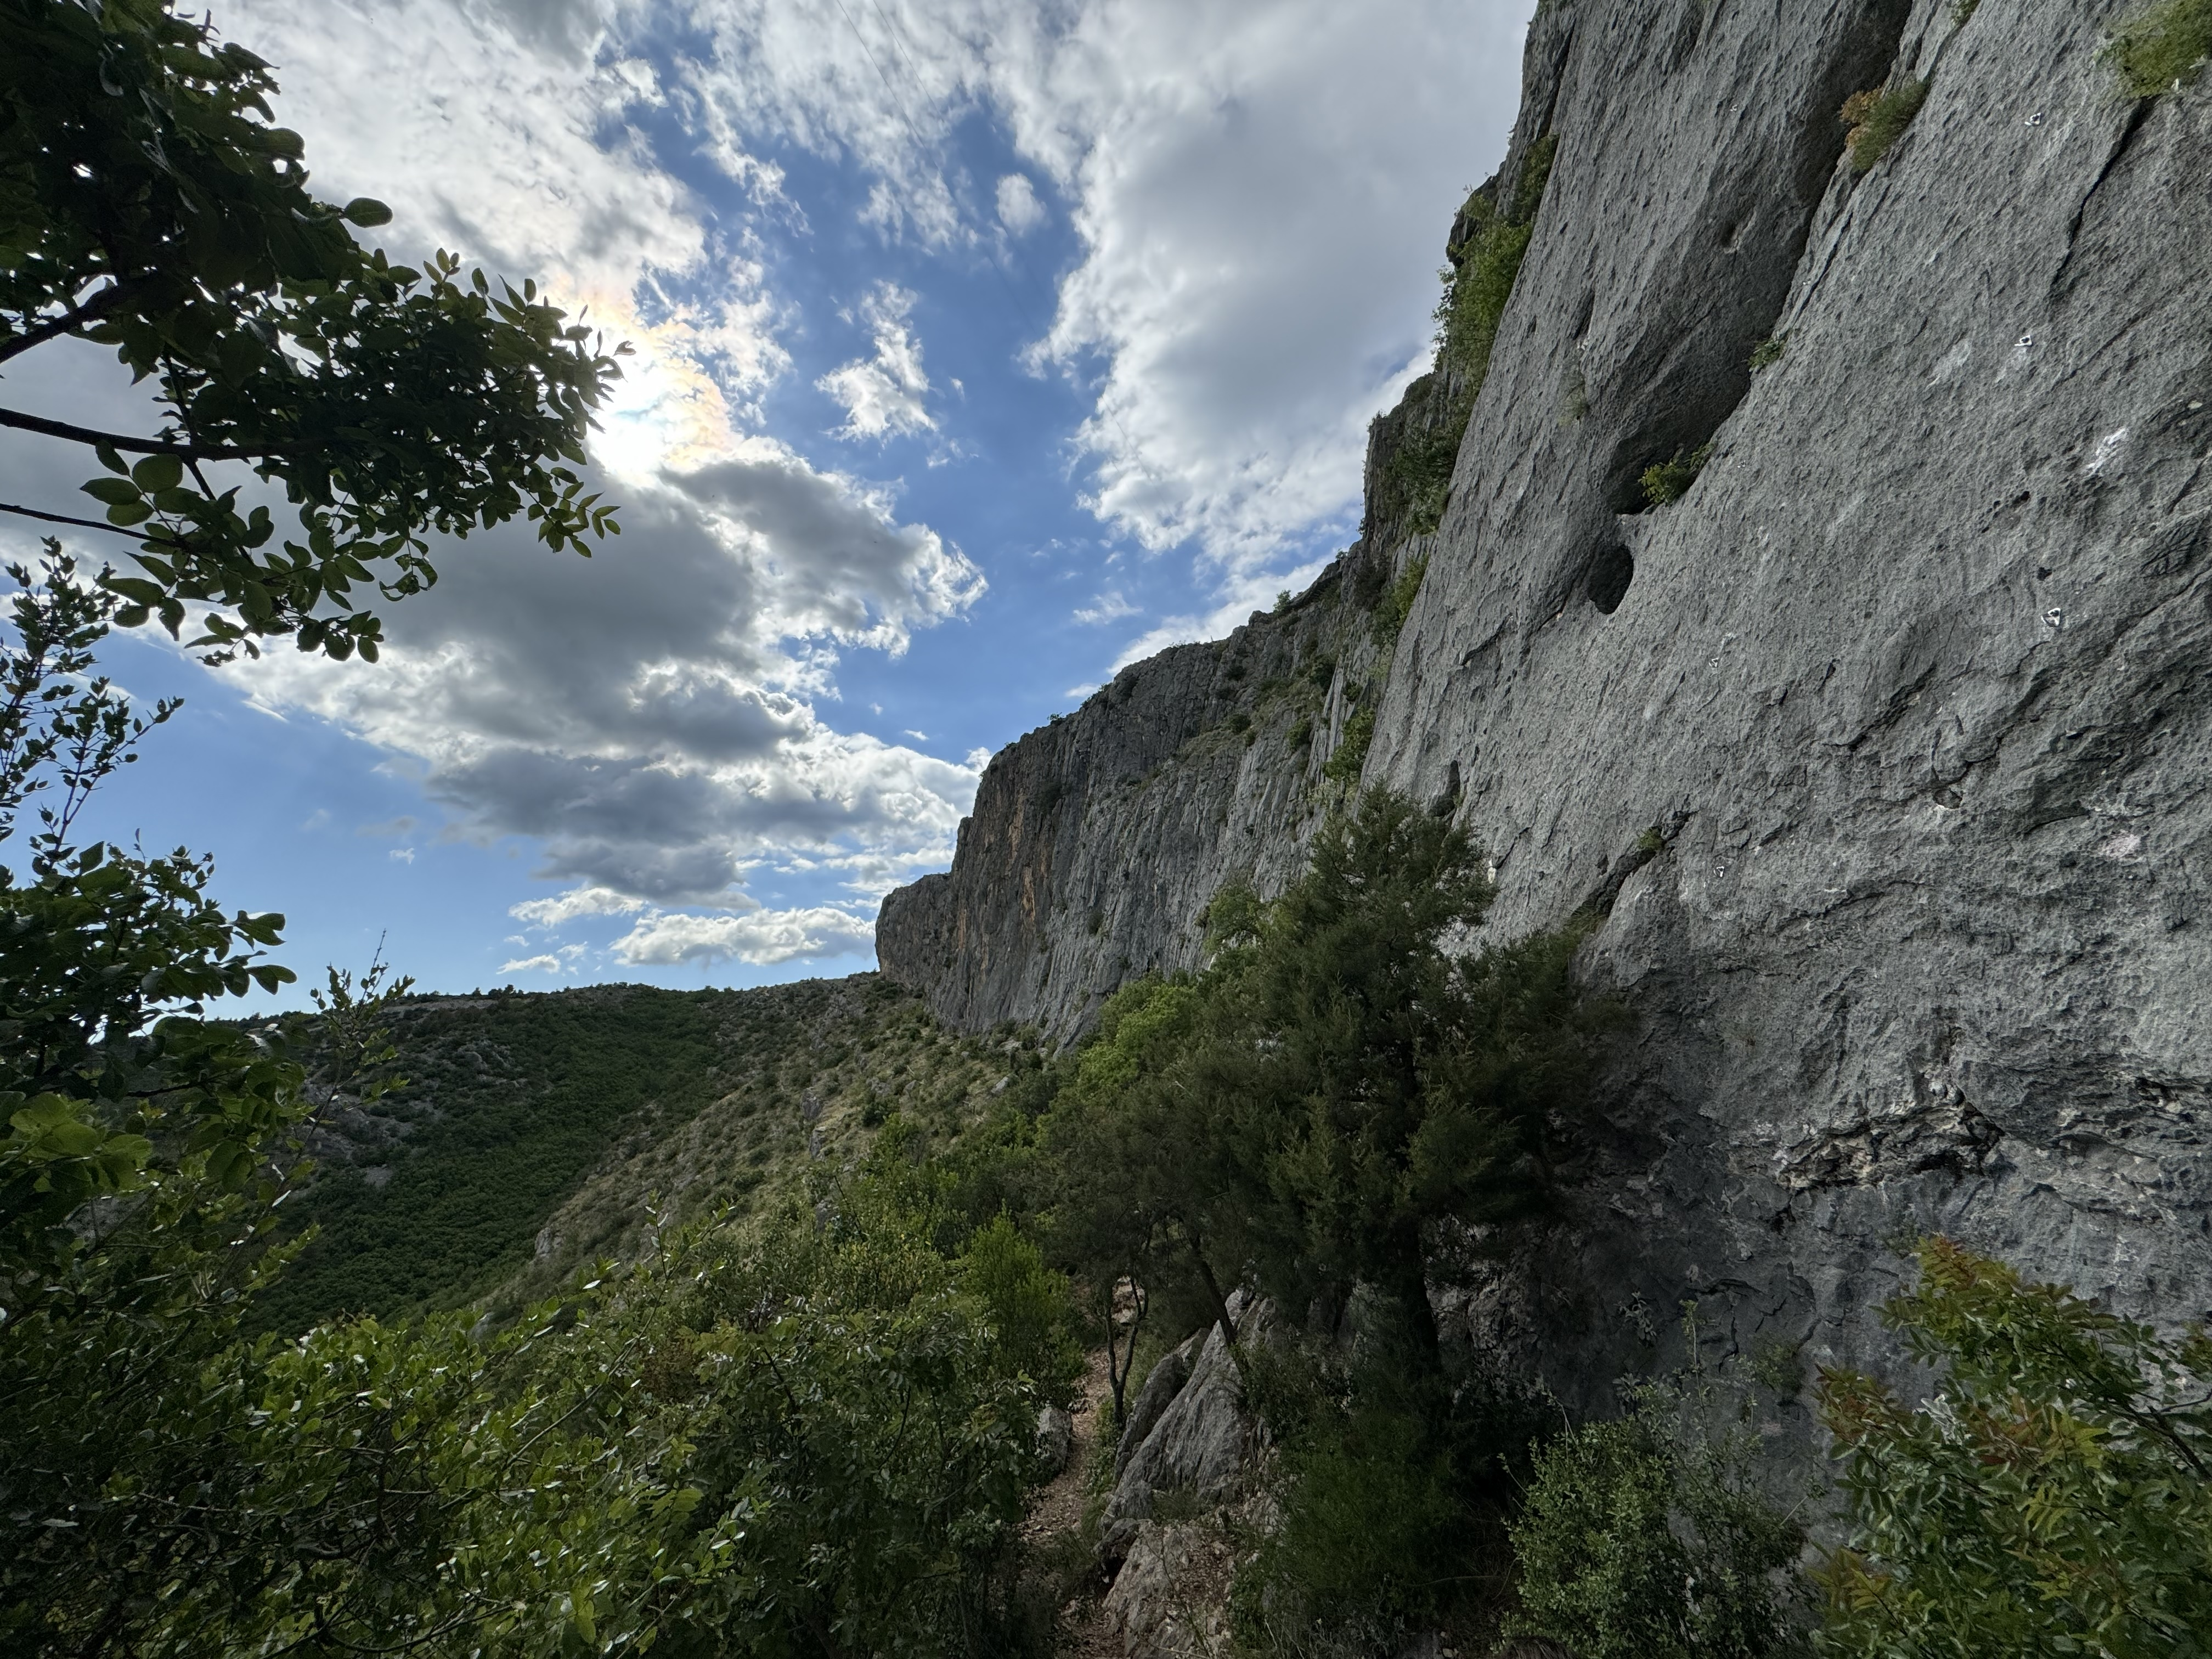
\includegraphics[width=0.38\textwidth]{images/uvod/cikola_fizicka_slika.jpg}
    \caption{Stvarna stijena na penjalištu Čikola sektora Osoje}
\end{figure}

\section{Cilj i doprinos rada}

Navedeni nedostaci postojećih alata stvaraju potrebu za rješenjem koje pokriva njihove nedostatke. Cilj je iskoristiti mobilnu tehnologiju kako bi se stvorilo rješenje koje bi minimiziralo navedene nedostatke. Ideja je omogućiti penjačima da jednostavnim usmjeravanjem kamere mobilnog uređaja prema stijeni dobije vizualnu informaciju o položaju i nazivima smjerova izravno u stvarnom okruženju korištenjem tehnologije proširene stvarnosti. Takav pristup ne samo da štedi vrijeme i smanjuje frustracije, već i omogućuje sigurnije iskustvo penjanja.


% \input{sections/Uvod/subsections/problem.tex}
% \input{sections/Uvod/subsections/cilj_rada.tex}


\chapter{Zaključak}

\section{Sažetak rada i ostvareni rezultati}

Problem identifikacije penjačkih smjerova na terenu, koji proizlazi iz ograničenja tradicionalnih tiskanih i postojećih digitalnih vodiča, predstavljao je temeljnu motivaciju za ovaj diplomski rad. Cilj je bio implementirati cjelovit softverski sustav "Alpinity" koji koristi tehnologije računalnog vida i proširene stvarnosti kako bi riješio taj problem.

Uz rad razvijen je i funkcionalni digitalni penjački vodič koji se sastoji od pozadinskog sustava, web aplikacije i mobilne aplikacije za iOS. Implementirana je funkcionalnost koja korisniku omogućuje da, usmjeravanjem kamere prema stijeni, u stvarnom vremenu dobije vizualnu informaciju o položaju penjačkog smjera. Testiranje u realnim uvjetima potvrdilo je da je odabrani algoritamski pristup, temeljen na detekciji značajki pomoću SIFT algoritma i procjeni homografije, funkcionalan i sposoban za prepoznavanje smjerova s različitim vizualnim karakteristikama.

Međutim, testiranje i vrednovanje je također otkrilo i ograničenja implementacije, prvenstveno u vidu latencije i povremene nestabilnosti detekcije, što je posljedica računskog opterećenja na mobilnom uređaju. Unatoč tim ograničenjima, rad je demonstrirao da je koncept vizualizacije smjerova pomoću proširene stvarnosti izvediv i da nudi potencijal za unapređenje korisničkog iskustva digitalnih penjačkih vodiča.

\section{Smjernice za budući razvoj}

\subsection{Poboljšanja procesa prepoznavanja}

Iako je razvijeni sustav funkcionalan, postoji prostor za daljnja poboljšanja. U nastavku se razmatraju područja za budući razvoj, s posebnim naglaskom na unapređenje procesa prepoznavanja.

Uočeni problemi latencije i vizualnog šuma mogu se ublažiti implementacijom optimizacija. Namještanjem parametara za SIFT algoritam i povećanjem minimalnog broja potrebnih parova značajki mogli bi pojačati preciznost detekcije i smanjiti vizualni šum. Trenutni sustav izračunava homografiju neovisno za svaki obrađeni kadar, što može dovesti do nestabilnosti i pogrešne detekcije. U budućnosti bi se moglo implementirati provjera koeficijenta matrice homografije kako bi se osiguralo da matrica ne transformira sliku u nestvarne oblike ili koristeći druge apstraktnije metode provjere matrice. Ako je dobivena matrica pala te testove onda se ne bi koristila za transformaciju slike i time se ne bi detektirala linija penjačkog smjera.

Nadalje, obrada zamućenih kadrova, nastalih brzim pokretom kamere, bespotrebno troši resurse i može dovesti do pogrešnih podudaranosti. Moguće je implementirati pred-procesni korak za filtriranje zamućenih kadrova. Primjerice, izračunom varijance Laplaceove transformacije slike može se procjeniti razina oštrine, te bi se kadrovi koji ne zadovoljavaju minimalni prag oštrine mogli ne dodati u spremnik kadrova i time ne bi se slali na obradu pomoću SIFT algoritma.

Konačno, trenutna arhitektura dizajnirana je za prepoznavanje jednog, unaprijed odabranog smjera. Značajno unapređenje bilo bi omogućiti sustavu detekciju više smjerova, recimo jednog sektora, istovremeno. To bi zahtijevalo da se deskriptori s kamere uspoređuju s cjelokupnom bazom deskriptora za sve smjerove u sektoru. Iako je ovo računski znatno zahtjevnije, pružilo bi bolje korisničko iskustvo.

\subsection{Integracija topografskih prikaza}


Testiranje je pokazalo da su referentne slike snimljene sa tla korisne za identifikaciju početka smjera, ali često ne mogu obuhvatiti cijeli tijek smjera, pogotovo kod dužih smjerova. S druge strane, klasične topo skice, iako apstraktne, pružaju jasan pregled cijele linije. Budući razvoj mogao bi uključivati hibridni pristup. Nakon što aplikacija uspješno prepozna penjački smjer, korisniku bi se mogla ponuditi opcija prebacivanja na 2D topo prikaz tog sektora, s jasno istaknutim prepoznatim smjerom. Time bi se kombinirale prednosti oba svijeta, precizna identifikacija na terenu i jasan pregled cijelog smjera pomoću topografske skice.



% \bibliography{literatura}
% \bibliographystyle{fer}

% %! Author = acvijanovic
%! Date = 10.06.2023.

\begin{thebibliography}{9}
    \bibitem{whatis_ieee80211}
    Samsung, What is IEEE 802.11 Wireless LAN(WLAN) technology?
    (2020, listopad).

    Poveznica: https://www.samsung.com/in/support/mobile-devices/what-is-ieee-802-11-wireless-lan-wlan-technology/;
    pristupljeno 30. svibnja 2023.

    \bibitem{difference_wifi_wlan}
    Lee Badman, What is the difference between WLAN and Wi-Fi?

    Poveznica: https://www.techtarget.com/searchnetworking/answer/Wireless-vs-Wi-Fi-What-is-the-difference-between-Wi-Fi-and-WLAN;
    pristupljeno 30. svibnja 2023.
\end{thebibliography}

% 
\begin{sazetak}
    Sažetak na hrvatskom jeziku.
    
    \kljucnerijeci{Ključne riječi, odvojene zarezima.}
    \end{sazetak}
    
    % TODO: Navedite naslov na engleskom jeziku.
    \engtitle{An application for interactive assistance to rock climbers using augmented reality}
    \begin{abstract}
    Abstract.
    
    \keywords{Keywords.}
    \end{abstract}



\end{document}
